\expandafter\let\csname ver@amssymb.sty\endcsname\empty
\documentclass[serif]{beamer}
\expandafter\let\csname ver@amssymb.sty\endcsname\relax

\usepackage[bitstream-charter]{mathdesign} % Use BT Charter font
\usepackage[T1]{fontenc}                   % Use T1 encoding instead of OT1
\usepackage[utf8]{inputenc}                % Use UTF8 input encoding
\usepackage{microtype}                     % Improve typography
\usepackage{booktabs}
\usepackage{cancel}
\usepackage{algorithm}
\usepackage{algorithmicx}
\usepackage{algpseudocode}
\usepackage{hyperref}
\hypersetup{pdfstartview=Fit}
\usepackage{xcolor}
\usepackage{tikz}
\usepackage{tikz-qtree}

\usetheme{Berlin}
\usecolortheme{beaver}

\title{Lecture 19 --- 4th Order Generalized Runge Kutta Methods w/ Automatic Time Step Adjustment}
\author{Bryan R. Herman}
\date{November 21, 2012}

% \AtBeginSection[]
% {
%   \begin{frame}<beamer>
%     \frametitle{Outline}
%     \tableofcontents[currentsection]
%   \end{frame}
% }
% \beamerdefaultoverlayspecification{<+->}

\renewcommand{\algorithmicforall}{\textbf{for each}}

\usenavigationsymbolstemplate{}

% -----------------------------------------------------------------------------
\begin{document}

\frame{\titlepage}

\begin{frame}{Goals of today's lecture}
  \begin{enumerate}
  \item<1-> Derivation of Generalized Runge Kutta (GRK) methods is complicated
            --- Hopefully I can make some sense of it for you!
  \vfill
  \item<1-> Implementation of GRK methods is not difficult --- Hopefully you
            can go home and implement this.
  \vfill
  \item<1-> Automatic time step adjustment is easy with certain RK methods ---
            Basically comes for free.
  \end{enumerate}
\end{frame}

% -----------------------------------------------------------------------------
\section{Introduction}

\begin{frame}{The need for higher order methods}
  \begin{itemize}
  \item<1-> To get accurate results with implicit methods must use fine time steps
  \vfill
  \item<1-> Higher order methods allow for larger time step, more expensive
  \vfill
  \item<1-> 4-th order GRK methods allow are semi-implicit and relatively stable
  \vfill
  \item<1-> Embedded truncation error estimation allows for informed adjustments
            of time step
  \end{itemize}
\end{frame}

\begin{frame}{What are we trying to solve}
  \begin{equation}
    \nonumber \mathbf{y}^\prime\left(t\right) = \mathbf{f}\left(t,\mathbf{y}\left(t\right)\right)
  \end{equation}
  \vfill
  What methods do we have to solve this ---
  \vfill
  \begin{itemize}
   \item<1-> Single-step methods --- Euler methods, \color<2->{blue} Runge Kutta Methods\color<1->{black}, ...
   \vfill
   \item<1-> Multi-step methods  --- Adams-Bashforth, Adams-Moulton, BDF methods ....
  \item<2-> All forms of {\color{blue}{Runge Kutta}} get the next time step values with:
  \begin{equation}
    \nonumber \mathbf{y}^{n+1} = \mathbf{y}^n + \sum_{i=1}^s m_i \mathbf{k}_i
  \end{equation}
  \begin{center}
    \color{red}{All the work goes into determining $k$ parameters}
  \end{center}
  \end{itemize}
\end{frame}

%--------------------------------------------------------------------------------
\section{Runge Kutta Methods}

\begin{frame}{Autonomous Forms of Runge Kutta}
  \begin{itemize}
  \item<1-> Explicit Form
  \only<1>{\begin{equation}
   \nonumber \mathbf{k}_i = h\mathbf{f}\left(\mathbf{y}_n + \sum_{j=1}^{i-1}a_{ij}\mathbf{k}_j\right) 
  \end{equation}}
  \only<2->{\begin{equation}
    \nonumber \mathbf{k}_i = h\mathbf{f}\left(\mathbf{y}_n + \sum_{j=1}^{{\color{green!75!black}i-1}}a_{ij}\mathbf{k}_j\right) 
  \end{equation}}
  \item<1-> Implicit Form
  \only<1>{\begin{equation}
    \nonumber \mathbf{k}_i = h\mathbf{f}\left(\mathbf{y}_n + \sum_{j=1}^{s}a_{ij}\mathbf{k}_j\right) 
  \end{equation}}
  \only<2->{\begin{equation}
    \nonumber \mathbf{k}_i = h\mathbf{f}\left(y_n + \sum_{j=1}^{{\color{green!75!black}s}}a_{ij}\mathbf{k}_j\right) 
  \end{equation}}
  \item<1-> {\color<2->{green!75!black}  Diagonally Implicit Form}
  \only<1>{\begin{equation}
   \nonumber \mathbf{k}_i = h\mathbf{f}\left(\mathbf{y}_n + \sum_{j=1}^{i}a_{ij}\mathbf{k}_j\right) 
  \end{equation}}
  \only<2->{\begin{equation}
    \nonumber \mathbf{k}_i = h\mathbf{f}\left(\mathbf{y}_n + \sum_{j=1}^{{\color{green!75!black}i}}a_{ij}\mathbf{k}_j\right) 
  \end{equation}}
  \end{itemize}
\end{frame}

\begin{frame}{Removing nonlinearity from implicit form}
  \begin{itemize}
  \item<1-> The fully implicit form is difficult to solve since it nonlinearly depends on all values of $k$
  \item<1-> Instead, we use diagonally implicit form and linearize
  \vfill
  \item<2->  We define $\mathbf{y}^\prime = \mathbf{y}_n + \sum_{j=1}^{i-1}a_{ij}\mathbf{k}_j$ such that
  \begin{equation}
    \nonumber \mathbf{k}_i = h\mathbf{f}\left(\mathbf{y}^\prime + a_{ii}\mathbf{k}_i\right) 
  \end{equation}
  \item<3-> Performing linearizeation about $\mathbf{y}^\prime$:
  \begin{equation}
   \nonumber \mathbf{k}_i = h\mathbf{f}\left(\mathbf{y}^\prime\right) + h\mathbb{J}\left(\mathbf{y}^\prime\right)a_{ii}\mathbf{k}_i
  \end{equation}
  \item<3-> \alert{Assumption:} Jacobian is not evaluated at intermediate time values
  \begin{equation}
   \nonumber \mathbf{k}_i = h\mathbf{f}\left(\mathbf{y}_n + \sum_{j=1}^{i-1}a_{ij}\mathbf{k}_j\right) + h\mathbb{J}\left(\mathbf{y}_n\right)a_{ii}\mathbf{k}_i
  \end{equation}
  \end{itemize}
\end{frame}

\begin{frame}{Rosenbrock form --- Generalized Runge Kutta}
  \begin{itemize}
  \item<1-> Change $a_{ii}$ to a linear combination ---
  \begin{equation}
    \nonumber \mathbf{k}_i = h\mathbf{f}\left(\mathbf{y}_n + \sum_{j=1}^{i-1}a_{ij}\mathbf{k}_j\right) +     
     h\mathbb{J}\left(\mathbf{y}_n\right)\color{blue}\sum_{j=1}^{i}c_{ij}\mathbf{k}_j
  \end{equation}
  \item<1-> System can be solved for each $\mathbf{k}_i$, next time step is
  \begin{equation}
  \nonumber \mathbf{y}^{n+1} = \mathbf{y}^n + \sum_{i=1}^s m_i \mathbf{k}_i
  \end{equation}
  \end{itemize}
  \begin{center}
    This is the autonomous form of the Rosenbrock equations. What if the right hand side depends on time (e.g. $\rho(t)$)?
  \end{center}
\end{frame}

\begin{frame}{Rosenbrock equations --- nonautonomous form (I)}
  If the differential equations are not autonomous, make $t$ another variable in the solution and derivative vector:
  \begin{equation}
    \nonumber \mathbf{y} = \left[ \begin{array}{c}
    \mathbf{y}_y \\
    t
    \end{array} \right ] \qquad
    \nonumber \mathbf{y}^\prime = \left[ \begin{array}{c}
    \mathbf{y}_y^\prime \\
    1
    \end{array} \right ]
  \end{equation}
  We can also define the Jacobian and the $k$-vector similarly
  \begin{equation}
    \nonumber \mathbb{J} = \left[ \begin{array}{cc}
    \mathbb{J}_{yy} & \mathbf{J}_{yt} \\
    0 & 0
    \end{array} \right]
  \end{equation}
  \begin{equation}
    \nonumber \mathbf{k}_i = \left[ \begin{array}{c}
    \mathbf{k}_{i,y} \\
    k_{i,t}
    \end{array} \right ]
  \end{equation}
\end{frame}

\begin{frame}{Rosenbrock equations --- nonautonomous form (II)}
  \begin{itemize}
  \item<1-> Writing out Rosenbrock equation:
  \end{itemize}
  \begin{equation}
    \nonumber\left[ \begin{array}{c}
    \mathbf{k}_{i,y} \\
    k_{i,t}
    \end{array} \right ] = h\left[ \begin{array}{c}
    \mathbf{f}_y\left(\mathbf{y}_n + \sum_{j=1}^{i-1}a_{ij}\mathbf{k}_{j,y}\right) \\
    f_t\left(t_n + \sum_{j=1}^{i-1}a_{ij}k_{j,t}\right) 
    \end{array} \right] +  h\left[ \begin{array}{cc}
        \mathbb{J}_{yy} & \mathbf{J}_{yt} \\
    0 & 0
    \end{array} \right]\sum_{j=1}^i c_{ij}\left[ \begin{array}{c}
    \mathbf{k}_{j,y} \\
    k_{j,t}
    \end{array} \right]
  \end{equation}
  \begin{itemize}
  \item<1-> Taking the second equation:
  \end{itemize}
  \vfill
  \begin{equation}
    \nonumber k_{i,t} = h f_t\left(t_n + \sum_{j=1}^{i-1}a_{ij}\mathbf{k}_{j,t}\right)
  \end{equation}
  \begin{itemize}
  \item<1-> The function evaulation of time derivative is always unity:
  \end{itemize}
  \vfill
  \begin{equation}
    \nonumber k_{i,t} = h
  \end{equation}
\end{frame}

\begin{frame}{Rosenbrock equations --- nonautonomous form (III)}
  \begin{itemize}
  \item<1-> Substituting $k_{i,t}$ into the first equations:
  \end{itemize}
  \begin{align*}
    \mathbf{k}_{i,y} = &  h\mathbf{f}_y \left(t_n + h\sum_{j=1}^{i-1}a_{ij},\mathbf{y}_n + \sum_{j=1}^{i-1}a_{ij}\mathbf{k}_{j,y}\right) \\
                                + & h\mathbb{J}_{yy}\sum_{j=1}^i c_{ij}\mathbf{k}_{j,y}  + \mathbf{J}_{yt}h\sum_{j=1}^i c_{ij}
  \end{align*}
  \begin{itemize}
  \item We drop the $y$ subscripts and can make the following definitions: 
  \end{itemize}
  \begin{equation}
    \nonumber d_i \equiv \sum_{j=1}^{i-1} a_{ij} \qquad  b_i \equiv \sum_{j=1}^i c_{ij} \qquad \frac{d\mathbf{f}}{dt} \equiv \mathbf{J}_{yt}
  \end{equation}
\end{frame}

\begin{frame}{Rosenbrock equations --- nonautonomous form (IV)}
  \begin{equation}
    \nonumber \mathbf{k}_{i} = h\mathbf{f} \left(t_n + d_ih,\mathbf{y}_n + \sum_{j=1}^{i-1}a_{ij}\mathbf{k}_{j}\right) 
                                + h\mathbb{J}\sum_{j=1}^i c_{ij}\mathbf{k}_{j}  + b_ih\frac{d\mathbf{f}}{dt}
  \end{equation}
  \begin{equation}
    \nonumber \mathbf{y}_{n+1} = \mathbf{y}_{n} + \sum_{i=1}^s m_i\mathbf{k}_i
  \end{equation}
  \vfill
  \begin{itemize}
  \item<1-> Parameters $m_i$, $a_{ij}$ and $c_{ij}$ are determined from equations of condition
  \item<1-> Parameters $b_i$ and $d_i$ are derived from $c_{ij}$ and $a_{ij}$, respectively
  \item<1-> \alert{Note:} $\mathbb{J}$ and $\frac{d\mathbf{f}}{dt}$ are only evaluated at beginning of timestep
  \end{itemize}
\end{frame}

%--------------------------------------------------------------------------------
\section{Coefficients}

\begin{frame}{Determining Runge Kutta Coefficients}
  \begin{itemize}
   \item<1->  Need to determine coefficients in Runge Kutta equations
   \item<1->  Two methods presented here:
   \begin{enumerate}
   \item<1->  Matching Taylor Series
   \item<1->  Butcher Series
   \end{enumerate}
  \vfill
  \item Consider 2nd order Runge Kutta model ---
  \end{itemize}
  \begin{equation}
    \nonumber \mathbf{y}_{n+1} = \mathbf{y}_n + m_1\mathbf{k}_1 + m_2\mathbf{k}_2
  \end{equation}
  \begin{equation}
    \nonumber \mathbf{k}_1 = h\mathbf{f}\left(t_n,\mathbf{y}_n\right)
  \end{equation}
  \begin{equation}
    \nonumber \mathbf{k}_2 = h\mathbf{f}\left(t_n + d_2h, \mathbf{y}_n + a_{21}\mathbf{k}_1\right)
  \end{equation}
  \vfill
  \begin{center}
    \alert{Note:} $d_1$ will be 0 from its definiton
  \end{center}
\end{frame}

\begin{frame}{Matching Taylor Series --- RK2 (I)}
  \begin{itemize}
  \item<1-> Write Taylor series for $\mathbf{y}_{n+1}$ from $\mathbf{y}_n$ past 2nd order
  \end{itemize}
  \begin{equation}
    \nonumber
    \mathbf{y}_{n+1} = \mathbf{y}_n + h\left.\frac{d\mathbf{y}}{dt}\right|_{t_n} + \frac{h^2}{2}\left.\frac{d^2\mathbf{y}}{dt^2}\right|_{t_n} + \mathcal{O}\left(h^3\right)
  \end{equation}
  \begin{itemize}
  \item<1-> Definining the following:
  \end{itemize}
  \begin{equation}
    \nonumber
    \frac{d\mathbf{y}}{dt} = \mathbf{f};\qquad
    \frac{d^2\mathbf{y}}{dt^2} = \frac{d\mathbf{f}}{dt} = \frac{\partial\mathbf{f}}{\partial t} +  \frac{\partial\mathbf{f}}{\partial \mathbf{y}} \frac{d\mathbf{y}}{d t} = \frac{\partial\mathbf{f}}{\partial t} +  \frac{\partial\mathbf{f}}{\partial \mathbf{y}} \mathbf{f}
  \end{equation}
  \begin{itemize}
  \item<1-> Taylor series becomes
  \end{itemize}
  \begin{equation}
    \nonumber
    \mathbf{y}_{n+1} = \mathbf{y}_n + h\mathbf{f}\left(t_n,\mathbf{y}_n\right) + \frac{h^2}{2}\left.\left(\frac{\partial\mathbf{f}}{\partial t} +  \frac{\partial\mathbf{f}}{\partial \mathbf{y}} \mathbf{f}\right)\right|_{\left(t_n,\mathbf{y}_n\right)}
  \end{equation}
\end{frame}

\begin{frame}{Matching Taylor Series --- RK2 (II)}
  \begin{itemize}
  \item<1-> Expand $k_2$ about $t_n$ and $\mathbf{y}_n$
  \end{itemize}
  \begin{align*}
    \mathbf{k}_2 = &  h\mathbf{f}\left(t_n + d_2h, \mathbf{y}_n + a_{21}\mathbf{k}_1\right) \\
              = &  h\mathbf{f}\left(t_n,\mathbf{y}_n\right) + d_2h^2\left.\frac{\partial\mathbf{f}}{\partial t}\right|_{\left(t_n,\mathbf{y}_n\right)} + a_{21}\mathbf{k}_1h\left.\frac{\partial\mathbf{f}}{\partial \mathbf{y}}\right|_{\left(t_n,\mathbf{y}_n\right)}
  \end{align*}
  \begin{itemize}
  \item<1-> Recall that $\mathbf{k}_1 = h\mathbf{f}\left(t_n,\mathbf{y}_n\right)$:
  \end{itemize}
  \begin{equation}
    \nonumber
    \mathbf{k}_2 =  h\mathbf{f}\left(t_n,\mathbf{y}_n\right) + h^2\left.\left(d_2\frac{\partial\mathbf{f}}{\partial t}+  a_{21}\frac{\partial\mathbf{f}}{\partial \mathbf{y}}\mathbf{f}\right)\right|_{\left(t_n,\mathbf{y}_n\right)}
  \end{equation}
\end{frame}

\begin{frame}{Matching Taylor Series --- RK2 (III)}
  \begin{itemize}
  \item<1-> Substitute $\mathbf{k}_1$ and $\mathbf{k}_2$ into $ \mathbf{y}_{n+1} = \mathbf{y}_n + m_1\mathbf{k}_1 + m_2\mathbf{k}_2$:
  \end{itemize}
  \begin{equation}
    \nonumber
    \mathbf{y}_{n+1} = \mathbf{y}_n + \left(m_1 + m_2\right)h\mathbf{f}\left(t_n,\mathbf{y}_n\right) + h^2\left.\left(m_2d_2\frac{\partial\mathbf{f}}{\partial t}+  m_2a_{21}\frac{\partial\mathbf{f}}{\partial \mathbf{y}}\mathbf{f}\right)\right|_{\left(t_n,\mathbf{y}_n\right)}
  \end{equation}
  \begin{itemize}
  \item<1-> Recall Taylor series result:
  \end{itemize}
  \begin{equation}
    \nonumber
    \mathbf{y}_{n+1} = \mathbf{y}_n + h\mathbf{f}\left(t_n,\mathbf{y}_n\right) + \frac{h^2}{2}\left.\left(\frac{\partial\mathbf{f}}{\partial t} +  \frac{\partial\mathbf{f}}{\partial \mathbf{y}} \mathbf{f}\right)\right|_{\left(t_n,\mathbf{y}_n\right)}
  \end{equation}
  \begin{itemize}
    \item<1-> The resulting coefficient equations are:
  \end{itemize}
  \begin{equation}
  \nonumber\boxed{
  m_1 + m_2 = 1; \qquad m_2d_2 = \frac{1}{2}; \qquad m_2a_{21} = \frac{1}{2}}
  \end{equation}
\end{frame}

\begin{frame}{Matching Taylor Series --- RK2 (IV)}
  \begin{itemize}
  \item<1-> \alert{Note:} There are 3 equations, but 4 coefficients
  \item<1-> You are free to choose 1 of the parameters, but this will affect how the method performs
  \vfill
  \item<1-> For midpoint method:
  \end{itemize}
  \begin{equation}
   \nonumber
    m_1 = 0;\qquad m_2 = 1;\qquad d_2 = \frac{1}{2};\qquad a_{21} = \frac{1}{2}
  \end{equation}
  \begin{equation}
   \nonumber
   \mathbf{y}_{n+1} = \mathbf{y}_n + h\mathbf{f}\left[t_n + \frac{1}{2}h,\mathbf{y}_n + \frac{1}{2}h\mathbf{f}\left(t_n,\mathbf{y}_n\right)\right]
  \end{equation}
  \begin{itemize}
  \vfill
  \item<1-> For Heun's method:
  \end{itemize}
  \begin{equation}
   \nonumber
    m_1 = \frac{1}{2};\qquad m_2 = \frac{1}{2};\qquad d_2 = 1;\qquad a_{21} = 	1
  \end{equation}
  \begin{equation}
   \nonumber
   \mathbf{y}_{n+1} = \mathbf{y}_n + h\left\{\frac{1}{2}\mathbf{f}\left(t_n,\mathbf{y}_n\right)+ \frac{1}{2}\mathbf{f}\left[t_n + h,\mathbf{y}_n + h\mathbf{f}\left(t_n,\mathbf{y}_n\right)\right]\right\}
  \end{equation}
\end{frame}

\begin{frame}{Taylor Series matching is complicated}
  \begin{itemize}
  \item<1-> As higher order derivatives are needed, expressions get complicated to derive
  \item<1-> The first few derivatives are listed below:
  \end{itemize}
  \begin{equation}
    \nonumber
    \mathbf{y}^\prime\left(t\right) = \mathbf{f}\left[\mathbf{y}\left(t\right)\right]
  \end{equation}
  \begin{equation}
    \nonumber
    \mathbf{y}^{\prime\prime}\left(t\right) = \mathbf{f}^\prime\left[\mathbf{y}\left(t\right)\right]=\frac{d\mathbf{f}}{d\mathbf{y}}\frac{d\mathbf{y}}{dt} = \frac{d\mathbf{f}}{d\mathbf{y}}\mathbf{f}\left[\mathbf{y}\left(t\right)\right]
  \end{equation}
  \begin{align*}
    \mathbf{y}^{\prime\prime\prime}\left(t\right) = \mathbf{f}^{\prime\prime}\left[\mathbf{y}\left(t\right)\right]= & \frac{d^2\mathbf{f}}{d^2\mathbf{y}}\left(\frac{d\mathbf{y}}{dt}\right)^2 + \frac{d\mathbf{f}}{d\mathbf{y}} \frac{d^2\mathbf{y}}{dt^2} \\
    = & \frac{d^2\mathbf{f}}{d^2\mathbf{y}}\left(\frac{d\mathbf{y}}{dt}\right)^2 + \frac{d\mathbf{f}}{d\mathbf{y}} \frac{d\mathbf{f}}{d\mathbf{y}}\mathbf{f}\left[\mathbf{y}\left(t\right)\right]
  \end{align*}
\end{frame}

\begin{frame}{Patterns represented by rooted trees}
  \begin{itemize}
  \item<1-> We need to come up with a pattern for expressing derivatives --- rooted trees (Faa di Bruno formula w/ Bell polynomials)
  \end{itemize}
  \vfill
  \begin{columns}[t]
  \column{0.5\linewidth}
  \begin{equation}
    \nonumber
    \mathbf{y}^\prime\left(t\right) = \mathbf{f}\left[\mathbf{y}\left(t\right)\right]
  \end{equation} \vspace{0.05cm}
  \begin{equation}
    \nonumber
    \mathbf{y}^{\prime\prime}\left(t\right) = \frac{d\mathbf{f}}{d\mathbf{y}}\frac{d\mathbf{y}}{dt} = \frac{d\mathbf{f}}{d\mathbf{y}}\mathbf{f}\left[\mathbf{y}\left(t\right)\right]
  \end{equation} \vspace{-0.3cm}
  \begin{align*}
    \mathbf{y}^{\prime\prime\prime}\left(t\right) = & \frac{d^2\mathbf{f}}{d^2\mathbf{y}}\left(\frac{d\mathbf{y}}{dt}\right)^2 + \frac{d\mathbf{f}}{d\mathbf{y}} \frac{d^2\mathbf{y}}{dt^2} \\
    = & \frac{d^2\mathbf{f}}{d^2\mathbf{y}}\underbrace{\left(\frac{d\mathbf{y}}{dt}\right)^2}_{\mathrm{multi\,branch}} + \frac{d\mathbf{f}}{d\mathbf{y}} \underbrace{\frac{d\mathbf{f}}{d\mathbf{y}}\mathbf{f}\left[\mathbf{y}\left(t\right)\right]}_{\mathrm{single\,branch}}
  \end{align*}
  \column{0.5\linewidth}
  \begin{center}
  \vspace{-0.24cm}
  \begin{tikzpicture}
    \tikzstyle{every node}=[circle,draw,fill=black]
    \node {};
  \end{tikzpicture} \\ \vspace{.7cm}
  \begin{tikzpicture}
    \tikzset{level distance=20pt}
    \tikzset{sibling distance=72pt}
    \Tree [.\node[circle,draw,fill=black] {};  \node[circle,draw,fill=black] {}; ]
  \end{tikzpicture} \\ \vspace{0.7cm}
  \begin{tikzpicture}[grow'=up]
    \tikzset{level distance=20pt}
    \tikzset{sibling distance=20pt}
    \Tree [.\node[circle,draw,fill=black] {}; [.\node[circle,draw,fill=black] {};] [.\node[circle,draw,fill=black] {}; ] ]
  \end{tikzpicture} \hspace{0.2cm}
  \begin{tikzpicture}
    \tikzset{level distance=20pt}
    \tikzset{sibling distance=72pt}
    \Tree [.\node[circle,draw,fill=black] {};  [.\node[circle,draw,fill=black] {}; \node[circle,draw,fill=black] {};]]
  \end{tikzpicture} 
  \end{center}
  \end{columns}
\end{frame}

\begin{frame}{Rooted trees derived to 4th order}
\begin{center}
\scalebox{0.65}{
  \begin{tikzpicture}
    \tikzstyle{every node}=[circle,draw,fill=black,text=white]
    \node {1};
  \end{tikzpicture} \hspace{1cm}
  \begin{tikzpicture}
    \tikzset{level distance=40pt}
    \tikzset{sibling distance=72pt}
    \tikzstyle{every node}=[circle,draw,fill=black,text=white]
    \Tree [.\node {2};  \node {2}; ]
  \end{tikzpicture} \hspace{1cm}
  \begin{tikzpicture}[grow'=up]
    \tikzset{level distance=40pt}
    \tikzset{sibling distance=30pt}
    \tikzstyle{every node}=[circle,draw,fill=black,text=white]
    \Tree [.\node {3};  [.\node {3}; ] [.\node {3};] ]
  \end{tikzpicture} \hspace{1cm}
  \begin{tikzpicture}[grow'=up]
    \tikzset{level distance=40pt}
    \tikzset{sibling distance=30pt}
    \tikzstyle{every node}=[circle,draw,fill=black,text=white]
    \Tree [.\node {4};  [.\node {4};  \node {4};] ]
  \end{tikzpicture} \hspace{1cm}
  \begin{tikzpicture}[grow'=up]
    \tikzset{level distance=40pt}
    \tikzset{sibling distance=30pt}
    \tikzstyle{every node}=[circle,draw,fill=black,text=white]
    \Tree [.\node {5};  \node {5};  \node {5}; \node{5}; ]
  \end{tikzpicture}
} \\ \vspace{1cm}
\scalebox{0.65}{
  \begin{tikzpicture}[grow'=up]
    \tikzset{level distance=40pt}
    \tikzset{sibling distance=30pt}
    \tikzstyle{every node}=[circle,draw,fill=black,text=white]
    \Tree [.\node {6};  [.\node {6};  \node {6};] \node {6};  ]
  \end{tikzpicture} \hspace{1cm}
  \begin{tikzpicture}[grow'=up]
    \tikzset{level distance=40pt}
    \tikzset{sibling distance=30pt}
    \tikzstyle{every node}=[circle,draw,fill=black,text=white]
    \Tree [.\node {7};  [.\node {7};  \node {7}; \node {7};]  ]
  \end{tikzpicture} \hspace{1cm}
  \begin{tikzpicture}[grow'=up]
    \tikzset{level distance=40pt}
    \tikzset{sibling distance=30pt}
    \tikzstyle{every node}=[circle,draw,fill=black,text=white]
    \Tree [.\node {8};  [.\node {8};  [.\node {8}; [.\node {8};]]] ]
  \end{tikzpicture}
}
\end{center}
\end{frame}

\begin{frame}{Developing rooted trees is known as a Butcher Series}
  \begin{itemize}
    \item<1-> Recall Rosenbrock equations:
  \end{itemize}
  \begin{equation}
    \nonumber \mathbf{k}_{i} = h\mathbf{f} \left(t_n + d_ih,\mathbf{y}_n + \sum_{j=1}^{i-1}a_{ij}\mathbf{k}_{j}\right) 
                                + h\mathbb{J}\sum_{j=1}^i c_{ij}\mathbf{k}_{j}  + b_ih\frac{d\mathbf{f}}{dt}
  \end{equation}
  \begin{equation}
    \nonumber \mathbf{y}_{n+1} = \mathbf{y}_{n} + \sum_{i=1}^s m_i\mathbf{k}_i
  \end{equation}
  \begin{itemize}
  \item<1->  Parameters: $\mathbf{y}_n + \sum_{j=1}^{i-1}a_{ij}\mathbf{k}_{j}$, $\mathbf{y}_{n+1}$ and $\mathbf{k}_i$ can be represented with a Butcher series:
  \end{itemize}
  \begin{equation}
    \nonumber
    \mathbf{B}\left(\mathbf{a}, \mathbf{y}_0\right) = \sum_t \frac{h^{\rho\left(t\right)}}{\rho\left(t\right)!}\mathbf{a}\left(t\right)F\left(t\right)\mathbf{y}_0
  \end{equation}
  \begin{center}
    \alert{We will take an engineering approach to using Butcher Series}
  \end{center}
\end{frame}

\begin{frame}{Deriving Order Equations}
  \begin{itemize}
  \item<1-> We need to construct order equations of the form:
  \end{itemize}

  \begin{equation}
    \nonumber
    \sum_im_i\Phi_i\left(t\right)
  \end{equation}
  \begin{itemize}
  \item<1-> For $\Phi_i\left(t\right)$, we construct recursive formulas using the following notation for the types of roots in trees
      \begin{itemize}
      \item<1-> Type A: $a_{jk}$ whenver a multiple-branched node $j$ is directly connected with an upper node $k$
      \item<1-> Type B: $c_{jk}$ whenever a single-branched node $j$ is directly connected with an upper node $k$
      \end{itemize}
  \end{itemize}
  \begin{center}
  \scalebox{0.8}{
  \begin{tikzpicture}[grow'=up]
    \tikzset{level distance=40pt}
    \tikzset{sibling distance=30pt}
    \tikzstyle{every node}=[circle,draw,fill=black,text=white]
    \Tree [.\node {A};  [.\node[text=black] {A}; ] [.\node[text=black] {A};] ]
  \end{tikzpicture} \hspace{1cm}
  \begin{tikzpicture}[grow'=up]
    \tikzset{level distance=40pt}
    \tikzset{sibling distance=30pt}
    \tikzstyle{every node}=[circle,draw,fill=black,text=white]
    \Tree [.\node {B};  \node[text=black] {B}; ]
  \end{tikzpicture}
  }
  \end{center}
\end{frame}

\begin{frame}{Example 1 --- Setting up order equation of a tree}
  \begin{columns}[T]
  \column{0.75\linewidth}
  \begin{itemize}
  \item<1-> Consider the tree to the right
  \item<1-> Each node is labeled with a letter
  \item<1-> Node $k$ is Type A while $i$, $j$ and $m$ are Type B
  \item<1-> The order condition is:
  \end{itemize}
  \begin{equation}
    \nonumber
    \Phi_i\left(t\right) = c_{ij}c_{jk}a_{kl}a_{km}c_{mn}
  \end{equation}\vspace{-0.5cm}
  \begin{itemize}
  \item<1-> To simplify expressions can define:
  \end{itemize}
  \begin{equation}
    \nonumber
    a_i = \sum_j a_{ij} \qquad c_i = \sum_j c_{ij}
  \end{equation}\vspace{-0.5cm}
  \begin{itemize}
  \item<1-> Summation can be performed over maximal nodes $l$ and $n$:
  \end{itemize}
  \begin{equation}
    \nonumber
    \Phi_i\left(t\right) = c_{ij}c_{jk}a_{k}a_{km}c_{m}
  \end{equation}
  \column{0.25\linewidth}
  \vspace{0.8cm}
  \scalebox{0.8}{
  \begin{tikzpicture}[grow'=up]
    \tikzset{level distance=40pt}
    \tikzset{sibling distance=30pt}
    \tikzstyle{every node}=[circle,draw,fill=black,text=white]
    \Tree [.\node {i};  [.\node {j}; [.\node{k}; \node{l}; [.\node {m}; \node{n};]]]]
  \end{tikzpicture}}
  \end{columns}
\end{frame}

\begin{frame}{RHS of order conditions}
  \begin{itemize}
  \item<1-> The right hand side of the order equations is derived as:
  \end{itemize}
  \begin{equation}
    \nonumber
    \sum_im_i\Phi_i\left(t\right) = \sum_{j \geq 0} \left(-\gamma\right)^j\sum_{s\in V\left(s,j\right)} N\left(t,s\right)/\Gamma\left(s\right)
  \end{equation}
  \begin{itemize}
  \item<1-> The parmeters above are defined as:
    \begin{itemize}
    \item<1-> $V\left(s,j\right)$: a subtree $s$ that appears from tree $t$ by removing single-branched nodes; $j$ is the \# of nodes removed
    \item<1-> $N\left(t,s\right)$: number of possibilities to obtain $s$ by removing single-branched nodes from $t$
    \item <1-> $\Gamma\left(s\right)$ is defined recursively as:
    \end{itemize}
  \end{itemize}
  \begin{equation}
    \nonumber
    \Gamma\left(s\right) = \rho\left(s\right)\Gamma\left(s_1\right)...\Gamma\left(s_m\right)
  \end{equation}
  \begin{itemize}
  \item<1-> $\rho\left(s\right)$ is the number of nodes in tree $s$
  \item<1-> $s_m$ is a subtree obtained by removing $m$ roots of tree $s$
  \end{itemize}
\end{frame}

\begin{frame}{Example 2 --- RHS of tree (I)}
  \begin{columns}[T]
  \column{0.75\linewidth}
  \vspace{0cm}
  \begin{itemize}
  \item<1-> Black tree is original: $j=0$, $N\left(s,j\right)=1$, $\Gamma\left(s\right) = 6\cdot5\cdot4\cdot1\cdot2\cdot1$
  \vspace{0.1cm}
  \item<1-> {\color{red} Red tree} is original: $j=1$, $N\left(s,j\right)=2$, $\Gamma\left(s\right) = 5\cdot4\cdot1\cdot2\cdot1$
  \vspace{0.1cm}
  \item<1-> {\color{green} Green tree}: $j=1$, $N\left(s,j\right)=1$, $\Gamma\left(s\right) = 5\cdot4\cdot3\cdot1\cdot1$
  \vspace{0.1cm}
  \item<1-> {\color{orange} Orange tree}: $j=2$, $N\left(s,j\right)=2$, $\Gamma\left(s\right) = 4\cdot3\cdot1\cdot1$
  \vspace{0.1cm}
  \item<1-> {\color{blue} Blue tree}: $j=2$, $N\left(s,j\right)=1$, $\Gamma\left(s\right) = 4\cdot1\cdot2\cdot1$
  \vspace{0.2cm}
  \item<1-> {\color{purple} Purple tree}: $j=3$, $N\left(s,j\right)=1$, $\Gamma\left(s\right) =3\cdot1\cdot1$
  \end{itemize}
  \column{0.25\linewidth}
  \vspace{-0.3cm} 
  \begin{center}
  \scalebox{0.6}{
  \begin{tikzpicture}[grow'=up]
    \tikzset{level distance=20pt}
    \tikzset{sibling distance=10pt}
    \tikzstyle{every node}=[circle,draw,fill=black,text=white]
    \Tree [.\node {};  [.\node {}; [.\node{}; \node{}; [.\node {}; \node{};]]]]
  \end{tikzpicture}}  \hspace{0.5cm}
  \scalebox{0.6}{
  \begin{tikzpicture}[grow'=up]
    \tikzset{level distance=20pt}
    \tikzset{sibling distance=10pt}
    \tikzstyle{every node}=[circle,draw,fill=red,text=white]
    \Tree [.\node {}; [.\node{}; \node{}; [.\node {}; \node{};]]]
  \end{tikzpicture}} \\ \vspace{0.5cm}
  \scalebox{0.6}{
  \begin{tikzpicture}[grow'=up]
    \tikzset{level distance=20pt}
    \tikzset{sibling distance=10pt}
    \tikzstyle{every node}=[circle,draw,fill=green,text=white]
    \Tree [.\node {};  [.\node {}; [.\node{}; \node{}; [.\node {};]]]]
  \end{tikzpicture}}  \hspace{0.5cm}
  \scalebox{0.6}{
  \begin{tikzpicture}[grow'=up]
    \tikzset{level distance=20pt}
    \tikzset{sibling distance=10pt}
    \tikzstyle{every node}=[circle,draw,fill=orange,text=white]
    \Tree [.\node {}; [.\node{}; \node{}; [.\node {};]]]
  \end{tikzpicture}} \\ \vspace{0.5cm}
  \scalebox{0.6}{
  \begin{tikzpicture}[grow'=up]
    \tikzset{level distance=20pt}
    \tikzset{sibling distance=10pt}
    \tikzstyle{every node}=[circle,draw,fill=blue,text=white]
    \Tree [.\node{}; \node{}; [.\node {}; \node{};]]
  \end{tikzpicture}} \hspace{0.5cm}
 \scalebox{0.6}{
  \begin{tikzpicture}[grow'=up]
    \tikzset{level distance=20pt}
    \tikzset{sibling distance=10pt}
    \tikzstyle{every node}=[circle,draw,fill=purple,text=white]
    \Tree [.\node{}; \node{}; [.\node {};]]
  \end{tikzpicture}}\\
  No more single branched nodes.
  \end{center}
  \end{columns}
\end{frame}

\begin{frame}{Example 2 --- RHS of tree (II)}
  \begin{itemize}
  \item<1->  The order condition for this tree is:
  \end{itemize}
  \begin{align*}
    \sum_{i,j,k,m} m_{i}c_{ij}c_{jk}a_{k}a_{km}c_{m} = &  \frac{1}{240} - \frac{2\gamma}{40} - \frac{\gamma}{60} + \frac{2\gamma^2}{12} + \frac{1\gamma^2}{8} - \frac{\gamma^3}{3} \\ 
      = & \frac{1}{240} - \frac{\gamma}{15} + \frac{7\gamma^2}{24} - \frac{\gamma^3}{3}
  \end{align*}
\end{frame}

\begin{frame}{Recall the rooted trees for 4th order Rosenbrock}
\begin{center}
\scalebox{0.65}{
  \begin{tikzpicture}
    \tikzstyle{every node}=[circle,draw,fill=black,text=white]
    \node {1};
  \end{tikzpicture} \hspace{1cm}
  \begin{tikzpicture}
    \tikzset{level distance=40pt}
    \tikzset{sibling distance=72pt}
    \tikzstyle{every node}=[circle,draw,fill=black,text=white]
    \Tree [.\node {2};  \node {2}; ]
  \end{tikzpicture} \hspace{1cm}
  \begin{tikzpicture}[grow'=up]
    \tikzset{level distance=40pt}
    \tikzset{sibling distance=30pt}
    \tikzstyle{every node}=[circle,draw,fill=black,text=white]
    \Tree [.\node {3};  [.\node {3}; ] [.\node {3};] ]
  \end{tikzpicture} \hspace{1cm}
  \begin{tikzpicture}[grow'=up]
    \tikzset{level distance=40pt}
    \tikzset{sibling distance=30pt}
    \tikzstyle{every node}=[circle,draw,fill=black,text=white]
    \Tree [.\node {4};  [.\node {4};  \node {4};] ]
  \end{tikzpicture} \hspace{1cm}
  \begin{tikzpicture}[grow'=up]
    \tikzset{level distance=40pt}
    \tikzset{sibling distance=30pt}
    \tikzstyle{every node}=[circle,draw,fill=black,text=white]
    \Tree [.\node {5};  \node {5};  \node {5}; \node{5}; ]
  \end{tikzpicture}
} \\ \vspace{1cm}
\scalebox{0.65}{
  \begin{tikzpicture}[grow'=up]
    \tikzset{level distance=40pt}
    \tikzset{sibling distance=30pt}
    \tikzstyle{every node}=[circle,draw,fill=black,text=white]
    \Tree [.\node {6};  [.\node {6};  \node {6};] \node {6};  ]
  \end{tikzpicture} \hspace{1cm}
  \begin{tikzpicture}[grow'=up]
    \tikzset{level distance=40pt}
    \tikzset{sibling distance=30pt}
    \tikzstyle{every node}=[circle,draw,fill=black,text=white]
    \Tree [.\node {7};  [.\node {7};  \node {7}; \node {7};]  ]
  \end{tikzpicture} \hspace{1cm}
  \begin{tikzpicture}[grow'=up]
    \tikzset{level distance=40pt}
    \tikzset{sibling distance=30pt}
    \tikzstyle{every node}=[circle,draw,fill=black,text=white]
    \Tree [.\node {8};  [.\node {8};  [.\node {8}; [.\node {8};]]] ]
  \end{tikzpicture}
}
\end{center}
\end{frame}

\begin{frame}{Order Conditions up to 4th order}
  \begin{enumerate}
  \item<1-> $\sum m_i = 1 = p_1\left(\gamma\right)$
  \vfill
  \item<1-> $\sum m_ic_i = 1/2 - \gamma = p_2\left(\gamma\right)$
  \vfill
  \item<1-> $\sum m_ia_i^2 = 1/3 = p_3\left(\gamma\right)$
  \vfill
  \item<1-> $\sum m_ic_{ij}c_j = 1/6 - \gamma + \gamma^2 = p_4\left(\gamma\right)$
  \vfill
  \item<1-> $\sum m_ia_i^3 = 1/4 = p_5\left(\gamma\right)$
  \vfill
  \item<1-> $\sum m_ia_ia_{ij}c_j = 1/8 - \gamma/3 = p_6\left(\gamma\right)$
  \vfill
  \item<1-> $\sum m_ic_{ij}a_j^2 = 1/12 - \gamma/3 = p_7\left(\gamma\right)$
  \vfill
  \item<1-> $\sum m_ic_{ij}c_{jk}c_{k} = 1/24 - \gamma/2 + 3\gamma^2/2 - \gamma^3 = p_8\left(\gamma\right)$
  \end{enumerate}
\end{frame}

%-------------------------------------------------------------------------------
\section{Implementation}

\begin{frame}{Numerically efficient form of Rosenbrock equations}
 
\end{frame}

\begin{frame}{Coefficients are changed to...}

\end{frame}

%-------------------------------------------------------------------------------
\section{Examples}

\begin{frame}{Nordheim-Fuchs Model (NFM)}
  \begin{itemize}
    \item Assuming no delayed neutrons and adiabatic heat up:
  \end{itemize}
  \begin{equation}
    \nonumber
    \frac{d}{dt}\left[\begin{array}{c}
                        P\left(t\right) \\
                        T_f\left(t\right)
                      \end{array}\right] =
                \left[\begin{array}{c}
                        \frac{\rho_0 - \alpha_f\left(T_f\left(t\right) - T_{f,0}\right) - \beta}{\Lambda}P\left(t\right) \\
                        \frac{1}{m_fc_f}P\left(t\right)
                      \end{array}\right]
  \end{equation}
  \begin{itemize}
   \item The reactivity at any time is;
  \end{itemize}
  \begin{equation}
    \nonumber
    \rho\left(t\right) = \rho_0 - \alpha_f\left(T_f\left(t\right) - T_{f,0}\right)
  \end{equation}
  \begin{itemize}
   \item The Jacobian of the system is:
  \end{itemize}
  \begin{equation}
    \nonumber
    \mathbb{J} = \left[\begin{array}{cc}
                         \frac{\rho_0 - \alpha_f\left(T_f\left(t\right) - T_{f,i}\right) - \beta}{\Lambda} & -\frac{\alpha_f}{\Lambda}P\left(t\right) \\
                         \frac{1}{m_fc_f} & 0
                       \end{array}\right]
  \end{equation}
\end{frame}

\begin{frame}{NFM has an analytic solution}

  \begin{equation}
    \nonumber
    \omega = \frac{\rho_0 - \beta}{\Lambda}
    \end{equation}
\vfill
  \begin{equation}
    \nonumber
    P\left(t\right) = \frac{\Lambda\omega^2m_fc_f}{2\alpha}\mathrm{sech}^2\left(\frac{\omega t}{2}\right)
  \end{equation}
\vfill
  \begin{equation}
    \nonumber
    T_f\left(t\right) = \frac{\Lambda\omega}{\alpha}\mathrm{tanh}\left(\frac{\omega t}{2}\right) + T_f\left(0\right)
  \end{equation}
\vfill
  \begin{equation}
    \nonumber
    \rho\left(t\right) = \rho\left(0\right) - \left(\rho_0 - \beta\right)\mathrm{tanh}\left(\frac{\omega t}{2}\right)
  \end{equation}
\vfill
  \begin{center}
    \alert{Note:} In NFM model, peak power is at time 0 seconds.
  \end{center}

\end{frame}


\begin{frame}{NFM Results --- numerical results agree well}
  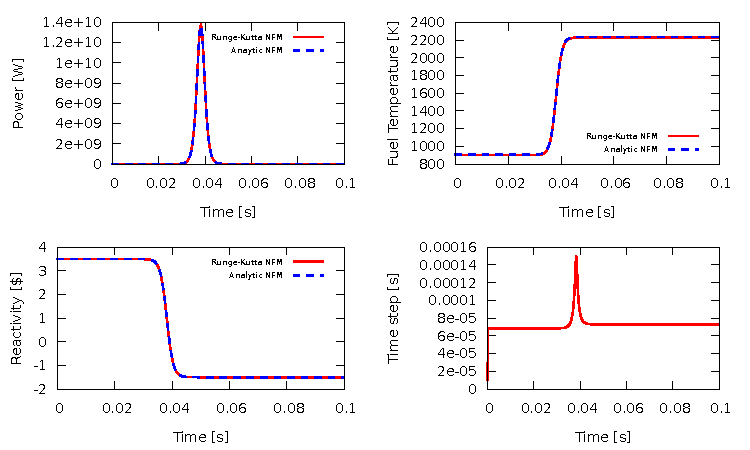
\includegraphics[scale=0.9]{./figs/nordheimfuchs.pdf}
\end{frame}

%--------------------------------------------------------------------------------
\end{document}
